\documentclass[whitelogo]{tudelft-report}
\usepackage{natbib}
\usepackage{changes}
\begin{document}

%% Use Roman numerals for the page numbers of the title pages and table of
%% contents.
\frontmatter

%% Uncomment following 19 lines for a cover with a picture on the lower half only
%\title[tudelft-white]{Title}
%\subtitle[tudelft-cyan]{Optional subtitle}
%\author[tudelft-white]{J.\ Random Author}
%\affiliation{Technische Universiteit Delft}
%\coverimage{cover.jpg}
%\titleoffsetx{10cm}
%\titleoffsety{10cm}
%\afiloffsetx{1cm}
%\afiloffsety{18cm}
%\covertext[tudelft-white]{
%    \textbf{Cover Text} \\
%    possibly \\
%    spanning 
%    multiple 
%    lines
%    \vfill
%    ISBN 000-00-0000-000-0
%}
%\makecover

%% Uncomment following 16 lines for a cover with a picture on the lower half only
\title[tudelft-white]{Plan of Action}
\subtitle[tudelft-black]{Quantifying numerical diffusion and dispersion in D-Flow Flexible Mesh using a lock-exchange experiment}
\author[tudelft-white]{D. Koetsenruijter}
\affiliation{Technische Universiteit Delft}
\coverimage{tank.jpg}
\covertext[tudelft-white]{
    \textbf{Bachelor Thesis, Department of Hydraulic Engineering} \\
    First supervisor: ir. L. Keyzer
    Second supervisor: Prof. dr. J. Pietrzak
    \vfill
    03-05-2020 
}
\setpagecolor{tudelft-cyan}
%\makecover[split]


%% Include an optional title page.
\begin{titlepage}


\begin{center}

%% Insert the TU Delft logo at the bottom of the page.

%% Print the title in cyan.
{\makeatletter
\largetitlestyle\fontsize{64}{94}\selectfont\@title
%\largetitlestyle\color{tudelft-cyan}\Huge\@title
\makeatother}

%% Print the optional subtitle in black.
{\makeatletter
\ifx\@subtitle\undefined\else
    \bigskip
   {\tudsffamily\fontsize{22}{32}\selectfont\@subtitle}    
    %\titlefont\titleshape\LARGE\@subtitle
\fi
\makeatother}

\bigskip
\bigskip

by
%door

\bigskip
\bigskip

%% Print the name of the author.
{\makeatletter
%\largetitlefont\Large\bfseries\@author
\largetitlestyle\fontsize{26}{26}\selectfont\@author
\makeatother}

\bigskip
\bigskip

%to obtain the degree of Master of Science
%ter verkrijging van de graad van Master of Science

%at the Delft University of Technology,
%aan de Technische Universiteit Delft,

%to be defended publicly on Tuesday January 1, 2013 at 10:00 AM.
%in het openbaar de verdedigen op dinsdag 1 januari om 10:00 uur.

\vfill

\begin{tabular}{lll}
    Student number: & 4332601 \\
    Project duration: & \multicolumn{2}{l}{April 20, 2020 -- June 12, 2020} \\
    Thesis committee:   & ir.\ L. \ Keyzer, & TU Delft, 1st supervisor \\
                        & Prof. \ dr.\ J.\ Pietrzak, & TU Delft, 2nd supervisor \\
\end{tabular}
%% Only include the following lines if confidentiality is applicable.

\bigskip
\bigskip
%\emph{This thesis is confidential and cannot be made public until December 31, 2013.}
%\emph{Op dit verslag is geheimhouding van toepassing tot en met 31 december 2013.}

\bigskip
\bigskip
%An electronic version of this thesis is available at \url{http://repository.tudelft.nl/}.
%\\[1cm]

%\centering{
\includegraphics{cover/logo_black}}


\end{center}

\begin{tikzpicture}[remember picture, overlay]
    \node at (current page.south)[anchor=south,inner sep=0pt]{
        
\includegraphics{cover/logo_black}
    };
\end{tikzpicture}

\end{titlepage}



%\chapter*{Preface}
\setheader{Preface}

Preface\ldots

\begin{flushright}
{\makeatletter\itshape
    \@author \\
    Delft, January 2013
\makeatother}
\end{flushright}



\tableofcontents

%% Use Arabic numerals for the page numbers of the chapters.
\mainmatter

\chapter{Introduction}\label{introduction}

Due to temperature and salinity differences density driven currents can
occur. Because important water systems such as the drinking water supply
and large coastal systems in the Netherlands are strongly influenced by
these currents it is important to understand these phenomena. With the
use of D-Flow FM, a software package by Deltares, the mixture of salt-
and fresh water can be numerically approximated. However, a side effect
of these numerical flow models is the occurrence of numerical diffusion
and dispersion caused by characteristics of the numerical discretization
scheme that is used.

Numerical diffusion is sometimes referred to as ``numerical viscosity''
since the associated approximation errors mimic the effect of an
increase in viscosity, i.e.~the solution is overdamped. Since viscous
properties of a fluid decrease the amplitude of the diffusivity rate in
advection-diffusion flow problems. Additionally, numerical dispersion is
related to unrealistic oscillations in an approximation of an
advection-diffusion problem that may occur if stability of the solution
is not ensured. Because avoiding such errors requires contrasting
measures a quantification of their responses to certain modelling
parameters is desirable.
\citep{zijlema_computational_2015, obrien_study_1950}

In order to quantify the numerical diffusion and dispersion terms in the
D-Flow FM model, and thus get an idea of the model's sensitivity to
certain parameters, a lock-exchange experiment will be set up which
serve as the basis for a sensitivity analysis. After an initial
qualitative analysis of the terms and settings found during an
explorative setup of the basic D-Flow FM model, a stable basis for the
parameter variations will be defined. In this basic model the desired
boundary conditions, the lenght and timescale of the simulation and the
constant parameters and modelling characteristics will be determined.
Herafter the creation of such basic model will be automated so that the
data required for the sensitivity analysis may be generated.

The required data consist of the numerical errors produced while
changing the grid resolution, the timestep size and parameters related
to the flow model. Subsequently the sensitivity S of a parameter P is
defined as the relative change of a state variable per change of this
parameter: S = (δx/x)/(δP/P). The state parameters are defined as the
difference between the approximation and the analytical solution at
predefined monitoring points, also known as the accuracy of the
approximation. Prematurely three state parameters are defined; the flow
velocity error, the density error and wave speed error.

During the explorative model setup and the data generation phase, the
observed data is analyzed and compared to certain indicator parameters
in order to explain the observed phenomena. These indicators have
previously been found to characterize the significance of certain
modelling parameters \citep{Shin2004} of a discretization scheme and the
associated error or are composites of important model parameter. Finally
the leverage of parameters, forcing functions and submodules of the
model are assessed based on the observed sensitivity for which a
possible explanation in terms of the indicators and model
characteristics will be sought.

This document describes the research questions and hypotheses in the
first chapter, subsequently it will describe the research strategy
explained above in further detail in chapter two. Lastly, in the
appendix a planning for this research project can be found.

\chapter{Research Question \&
Hypothesis}\label{research-question-hypothesis}

\subsection{Research questions}\label{research-questions}

\begin{enumerate}
\def\labelenumi{\arabic{enumi}.}
\tightlist
\item
  How much numerical diffusion and or dispersion does the D-Flow FM
  model produce when simulating a 3D lock-exchange experiment dependent?

  \begin{enumerate}
  \def\labelenumii{\arabic{enumii}.}
  \tightlist
  \item
    What is the order of errors produced by D-Flow FM as a result of
    numerical diffusion and/or dispersion?
  \item
    How sensitive is the accuracy of the D-Flow FM model to time, space
    and numerically related parameters?
  \item
    What sort of errors are produced given different parameters?
  \item
    What parameters in the D-Flow FM model have the largest influence on
    errors related to numerical diffusion and dispersion?
  \item
    Are there indicators that predict the occurrence of numerical
    diffusion and dispersion in D-Flow FM?
  \end{enumerate}
\end{enumerate}

\subsection{Hypotheses}\label{hypotheses}

\begin{enumerate}
\def\labelenumi{\arabic{enumi}.}
\tightlist
\item
  There is significant numerical diffusion and negligible numerical
  dispersion in the D-Flow FM model when performing a lock-exchange
  experiment.

  \begin{enumerate}
  \def\labelenumii{\arabic{enumii}.}
  \tightlist
  \item
    The order of errors is of 10E-4
  \item
    It is very sensitive to time and space related parameters and can be
    slightly improved by flow model parameters.
  \item
    Mostly numerical diffusion errors are produced except when more
    elaborate advection schemes are applied.
  \item
    The time step size, grid resolution and viscosity have the larges
    influence leverage on the accuracy of the model.
  \item
    Examples of such indicators are the dimensionless Reynolds and
    Froude numbers or the ratio between the net diffusivity coefficient
    in the model and the eddy
  \end{enumerate}
\end{enumerate}

\chapter{Model Exploration}\label{model-exploration}

In order to provide a solid basis for the sensitivity analysis the basic
model has to be applicable to the research objective and sufficiently
robust to enable all parameters to be explored. To ensure a working
model first most default settings will be used to set up the
lock-exchange model, this will already require a minimal definition file
where general settings, physics, geometry, flow and numerical parameters
are set.

Thereafter possibly more realistic physical properties, boundary
conditions, a more relevant geometry and specifics of the flow model
such as bed friction and the will be defined. This should be done with
the research objective in mind thus possibly requires setting up three
different models for three different mesh grids in order to enable
stable testing, at the cost of consistency between models. These
trade-offs with respect to the research applicability and
generalizability will have to be made.

Further on the post-processing of the generated model will be performed,
in this way the results of the basic model can be qualitatively assessed
with respect to basic indicators.

Finally, monitoring points have to be set up at logically sound
locations and the basic models and subsequent post-processing have to be
automated as much as possible.

In short the following parts of the model should be explored: 
\begin{verbatim}
- General settings

- Physics

- Geometry

- Flow

- Numerics

- Post-processing

- Automation
\end{verbatim}

\section{Boundary conditions}\label{boundary-conditions}

Choosing the correct boundary condition for the lock-exchange model may
be of significant importance considering the different boundary
conditions that can be chosen within D-Flow. These boundary conditions
can be divided into three groups and can all be related to the
lock-exchange quite well: - Boundary conditions that complement the
governing equations; continuity and momentum conservation. -
Supplementary boundary conditions that impose additional constraints at
a boundary. E.g. the weir at t=0 and the sidewalls and possibly the free
surface \citep{Adduce2012}. - Boundary conditions for constituents, such
as salinity.

\section{Hydrostatic characteristics}\label{hydrostatic-characteristics}

The model is hydrostatic thus vertical accelerations are not taken into
account. The pressure is assumed to vary linearly at each cell along the
vertical direction depending on the density state of the cell, related
to the temperature and salinity. \citep[p.121]{DFlowTechMan}

The horizontal stresses resulting from the vertical stress profile
however are included in the model. This should be further looked into.

\section{Bed level type}\label{bed-level-type}

Certain different bed level types may be specified that are either
piecewise constant (1,2) or piecewise linear (3-6).

\chapter{Data Generation}\label{data-generation}

In the third phase of the research, the research strategy is completely
developed and provides a way to generate the data required to test the
hypotheses, which is threefold and dependent on given parameter ranges:
- Analytical (exact) reference data at monitor points

\begin{verbatim}
- Results obtained from the model

- Indicator parameters based on the results and input parameters
\end{verbatim}

\subsection{State variables}\label{state-variables}

In order to define the sensitivity of the model to certain parameters,
the sensitivity S of a parameter P is defined as the relative change of
a state variable per change of this parameter: S = (δx/x)/(δP/P).

It seems that possibly one state variable would be enough which would be
the velocity. Yet it would be interesting to see if there is significant
molecular diffusion and thus measure the density as a state variable.
Also the negative and positive wave of the fluid with a higher density
will have a wave speed that might be to analyze because of it's possible
relation to the tide induced translatory wave in the Rhine-Muese delta.
- Flow velocity error

\begin{verbatim}
- Density error

- Wave speed error
\end{verbatim}

\textbf{It is also important to notice that it is still unknown how the
analytical solutions at the monitor points can be calculated.}

\subsection{Spacial sensitivity}\label{spacial-sensitivity}

A very important parameter in the flexible mesh is the resolution of the
grid and the sort of mesh used. In order to get a complete analysis of
numerical diffusion and dispersion errors in D-Flow FM this should be
elaborately evaluated. With respect to the grid three evaluation
criteria can be seperately evaluated to assess the applicability of the
results obtained from a model.

\begin{verbatim}
* Is the solution converging with an acceptable Residual RMS Error (< 10E-4)

* Are the imbalances of the results sufficiently small (< 1%)

* Achieve grid independence
\end{verbatim}

\subsubsection{Convergence \& grid
independency}\label{convergence-grid-independency}

Results obtained from the D-Flow FM model are the results of a numerical
approximation specific to the mesh grid defined in the posed problem.
Therefore the convergence of the solution and the independency of it's
results to the mesh grid needs to be analyzed.

With respect to convergence of the model the output can be analyzed
according to three points:

\begin{itemize}
\item
  Residual Mean Squared Error
\item
  Gradient at monitor points (and observed parameters)
\item
  Imbalance of the computation (Global sum of a parameter
\end{itemize}

A grid independence study is well depicted by plotting number of cells
vs.~value at monitoring points. However it may be expected that a
relatively acceptable tolerance might not be attained given the
limitations the numerical model poses on the grid size in combination
with the timestep and the viscosity.

\subsection{Numerical sensitivity}\label{numerical-sensitivity}

Another major parameter is the time step size of the approximation. The
discretized advection-diffusion equation can be found on page 43 of
\citet{DFlowTechMan}, which uses an implicit and explicit scheme.
Because of the explicit time integration of the momentum diffusion there
is a limitation on the time step, however, in D-Flow this is implemented
as a limitation on the eddy viscosity coefficient.

In general the turbulence and diffusion model parameters seems to have a
great influence on the calculation complexity of the model. Therefore in
appendix A an elaborate explanation of diffusion and turbulence
modelling is given including the way D-Flow FM deals with this. Because
turbulence, shear stresses and viscosity are similar processes all
expressed in diffusivity terms they are grouped in the appendix for
brevity.

In general the following parameters of the numerical model can be
evaluated: * Timestep (Δt)

\begin{verbatim}
* Viscosity

* Flow model parameters

    * Entrainment (mixing terms)

    * Turbulence parameters

* Numerical parameters 

    * Max. degree

    * Conditioner

    * Advection scheme
\end{verbatim}

\subsubsection{Numerical scheme}\label{numerical-scheme}

A short description of the numerical solving process implemented by
D-Flow can be explained as follows. The discretized PDE's are solved by
Gaussian elemination up to a maximum degree, a parameter that can be
set, after which the resulting diagonally dominant, symmetric matrix is
solved by the Conjugate Gradient method. Before the CG method is applied
the matrix is preconditioned in order to assure a fast convergence of
the CG method. Two methods can be used for this preconditioning: - Using
the Jacobi preconditioner the diagonally dominant matrix is
preconditioned by a matrix consisting only of the diagonal of the
original matrix. - Using the LU decomposition preconditioner lower- and
upper triangular matrices (L, U) are formed that enable a solving the
matrix by Ux = y and Ly = b. However these matrices may be a lot less
sparse then the original matrix which would cause an increase in memory
usage. To overcome this problem the maximum degree parameter in D-Flow
may be set.

\citep[ p.21]{DFlowTechMan}

(Possibly incomplete LUD is applied where L and U are matrices with a
same sparsity pattern as the original matrix are formed such that LU ≈
A. The matix M = LU is then used to precondition (L, U). The matix M =
LU is then used to precondition the original matrix before CG is
applied.)

\chapter{Data Analysis}\label{data-analysis}

\section{Indicator parameters}\label{indicator-parameters}

From phase 2 onwards the indicator parameters will be compared to the
obtained result in order to get insight into the model and how it
behaves. The following parameters will be used as indicators: 

\begin{verbatim}
* Reynolds number

* Froude number

* Diffusivity and viscosity (η = ρ∙D = ρ∙μ)
\end{verbatim}

\section{Numerical conditions}\label{numerical-conditions}

In order to analyze the numerical results and qualitatively be able to
explain why certain behaviour is observed the numerical schemes will be
analyzed according to common conditions and parameters used to asses the
consistency, stability and convergence of numerical methods and schemes.

\subsection{Consistency, stability and convergence of finite
differences}\label{consistency-stability-and-convergence-of-finite-differences}

\begin{enumerate}
\def\labelenumi{\arabic{enumi}.}
\item
  If the local truncation error goes to zero in the limit of Δx a finite
  difference scheme is called consistent.
\item
  If there exists a constant C independant of Δx such that the norm of
  matrix A stays smaller than C if Δx goes to zero, a finite differences
  scheme is called stable.
\item
  If the global truncation error goes to zero as Δx goes to zero a
  scheme is called convergent. This happens if the scheme is both
  consistent and stable.
\end{enumerate}

\citep{Vuik2007}

\subsection{Condition number}\label{condition-number}

The condition number Κ of a matrix A is defined as the ratio between the
relative error in the approximation (Δw/w) given a relative error in the
right hand side of the matrix equation (Δf/f). For symmetric matrices
this number is equal to the magnitude of the maximum eigenvalue divided
by the magnitude of the minimum eigenvalue: Κ =
\textbar{}λmax\textbar{}/\textbar{}λmin\textbar{}. This range of
eigenvalues can be estimated using Gershgorin circle theorem
\citep[p.107]{Vuik2007}.

Using a more realistic estimation of the relative error in the
approximation one can obtain the effective condition number defined as:
Κ-eff = 1/λmin ∙ \textbar{}f\textbar{}/\textbar{}w\textbar{}.

\subsection{Other conditions}\label{other-conditions}

The conditions below will be discussed further if they turn out to be
relevant.

\begin{verbatim}
* Von Neumann condition (Amplification factor)
* CFL condition (Positive numerical diffusion, domain of influence)
* Computational stability (Domain of influence)
* Heuristic stability 
* Monotonicity
\end{verbatim}

\citep{zijlema_computational_2015}

\subsection{Spectral analysis}\label{spectral-analysis}

If significant numerical dispersion is observed a spectral analysis may
be performed as proposed by \citet{Ruano2019}.

\subsection{Interval analysis}\label{interval-analysis}

To deal with uncertainties in model parameters an interval analysis may
be done. Also to attain a range of values for certain parameters.

\section{Variable leverage}\label{variable-leverage}

Eventually after the data analysis the sensitivity of the numerical
diffusion and dispersion produced by the model to a number of chosen
parameters can be produced. A distinction will be made between model
parameters, forcing and submodels in order to separate the grounds on
which conclusions can be drawn.

\begin{verbatim}
* Parameters

* Forcing 

* Submodels
\end{verbatim}


%% Use letters for the chapter numbers of the appendices.
\appendix

\chapter{Appendix A}\label{appendix-a}

\section{Modelling of flow and
transport}\label{modelling-of-flow-and-transport}

\subsection{Molecular diffusion}\label{molecular-diffusion}

As emphasized by \citep[p194]{Battjes2017}: ``..molecular diffusion is
irrelevant in civil engineering practice, where turbulent diffusion and
dispersion are dominant..''.

In this case however it could be relevant because of the specific
experiment. Still with the goal of modelling the Rhine-Maas delta in
mind emphasis may be put on diffusion and dispersion processes related
to turbulence.

\subsection{Turbulent diffusion}\label{turbulent-diffusion}

To describe the turbulent diffusion the fluctuating quantities are
averaged over a certain time and lenght scale. Because of gravity the
concentration gradient is positive in the downward z-direction. From the
averaging of the turbulent motion and the gravity induced concentration
gradient it follows, as quoted from \citep[p.197]{Vuik2007}, that:
``..turbulent fluctuations cause a mean transport in the direction of
decreasing values of the mean concentration, as in a diffusion
process.''

Because the fluctuating quantities cause such net transport processes,
the resulting motion and turbulent properties need to be quantified. To
this end \citet{Prandtl1925} defined the concept of mixing lenght that
defines the lenght over which the fluctuations cause a deviation from
the average state and correspond to the average distance the turbulence
eddies travel. For example, velocity fluctuations can be related to the
velocity of the turbulent eddies. Further the turbulence induced
transport processes are found to be proportional to the concentration
gradient, also called the turbulence diffusivity. It has the order of
magnitude of the eddie velocity times the mixing lenght.

For vertical diffusion in free surface flows the mixing lenght changes
over the depth since it is induced by the bed friction expressed in the
bed shear stress (τ-b). Using his an estimate of the particle velocity
can be made by the so-called shear velocity which together with a
parabolic variation of the mixing length over the depth gives a measure
for the turbulence diffusivity: εt = Κ∙u∙L = Κ∙u∙z∙(1 - z/d). Where Κ is
the Von Karman coefficient which was previously empirically determined.

In exactly this manner horizontal momentum can be vertically distributed
through so-called Reynolds shear stress (τ-xz). Thus, in this case it is
not a concentration (c) but a momentum per unit volume (ρu) that is
diffused, an effect referred to as eddy viscosity. In a simple free
surface flow \citep[p.199]{Vuik2007} shows how this leads to a
logarithmic velocity profile.

\section{Turbulence modelling in D-Flow
FM}\label{turbulence-modelling-in-d-flow-fm}

\subsection{Reynold stresses}\label{reynold-stresses}

In the D-Flow FM model the total horizontal viscosity can be divided
into three contributing parts: - sub grid scale turbulence - 3D
turbulence - dispersion for depth averaged simulation

\subsubsection{Horizontal eddy
viscosity}\label{horizontal-eddy-viscosity}

Modelling horizontal eddy viscosity has three seperate parameters that
determine the total viscosity as follow: μ-H = μ-sgs + μ-v + μ-H-back.

These three parameters account for the following: - Horizontal turbulent
viscosity may be underestimated because of the sub-grid scale turbulent
motions, i.e.~turbulence on a scale smaller than the meshgrid. This can
be resolved by the sub-grid scale viscosity: μ-sgs - With Reynolds
averaged shallow water equations horizontal eddy viscosity might not
accounted for (enough) either thus D-Flow introduces the μ-v. - If extra
constant or spatially dependant viscosity is desired the background
viscosity μ-back may be added.

With respect to the 3D viscosity resulting from three-dimensional
turbulence a closure model is used \citep[p.26]{DFlowTechMan}. For
specific closure models one can even account for unresolved mixing
through an ambient background mixing coefficient μ-V-back. Eventually
the vertical eddy viscosity is thus calculated by a combination of the
3D viscosity μ-v and μ-mol, the latter being the kinematic viscosity of
water, as follows: μ-v = μ-mol + max(μ-v, μ-v-back).

In D-Flow FM four turbulence closure models can be chosen, the first
being user defined and the latter three based on models by Kolmogorov
and Prandtl, all are explained in further detail in
\citep[p.112-120]{DFlowTechMan}; - Constant coefficient - resulting in a
parabolic vertical velocity profile - Algebraic eddy viscosity closure
model - based on the Von Karman constant (κ), the bed friction (Cf),
without including transport processes, computing mixing lenght (L), the
shear velocity and the vertical turbulent viscosity μ-v. - Κ-ε
turbulence model - involves solving a non-linear coupled system of
equations describing turbulent kinetic energy (Κ) and energy loss (ε)
including diffusivity coefficients (D), a turbulent kinetic energy
production term (P), a Buoyancy flux (B) and a variation of kalibration
terms (c1-3). Thereafter the vertical eddy viscosity μ-v is determined
as proportional to the ratio Κ²/ε and the mixing lenght. Still, this
coupled system has to be discretized in terms of advection and diffusion
which is done explicitly by a first order upwind scheme and implicitly,
respectively. Accordingly the production and buoyancy term are
discretized while conserving the diagonally dominant matrix (ensuring
positivity). Finally this leads to two tri-diagonal matrices for Κ and ε
that can be solved using Thomas algorithm, which may be seen as the
tri-diagonal LU-decomposition, by using specific boundary conditions. -
Κ-τ turbulence - Where τ is a typical timescale of the turbulent eddies
and the eddy viscosity is proportional to Κ∙τ. Coupled by a system of
convection diffusion equations including diffusivity, production and
buoyancy terms. The resulting advection equation is discretized with an
first order upwind difference scheme and the vertical diffusion term is
discretized implicitly by a temporal discretization scheme. Again this
leads to two tri-diagonal matrices that can be solved by the Thomas
algorithm using specific boundary conditions.

\chapter{Appendix B}\label{appendix-b}
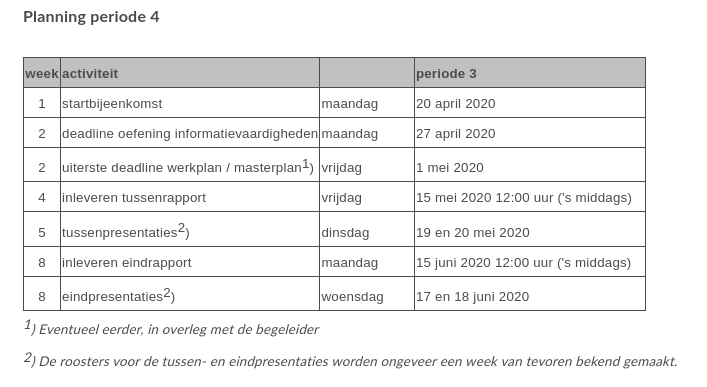
\includegraphics{/mnt/c/Users/daank/civiel/BEP/working/planofaction/planning.png}


%\input{appendix-a}

\bibliography{report}

\end{document}

